\begin{center}
    \textbf{Geração 1000}
\end{center}

\begin{figure}[h]
    \centering
    \label{fig:geracaoXX}
    
    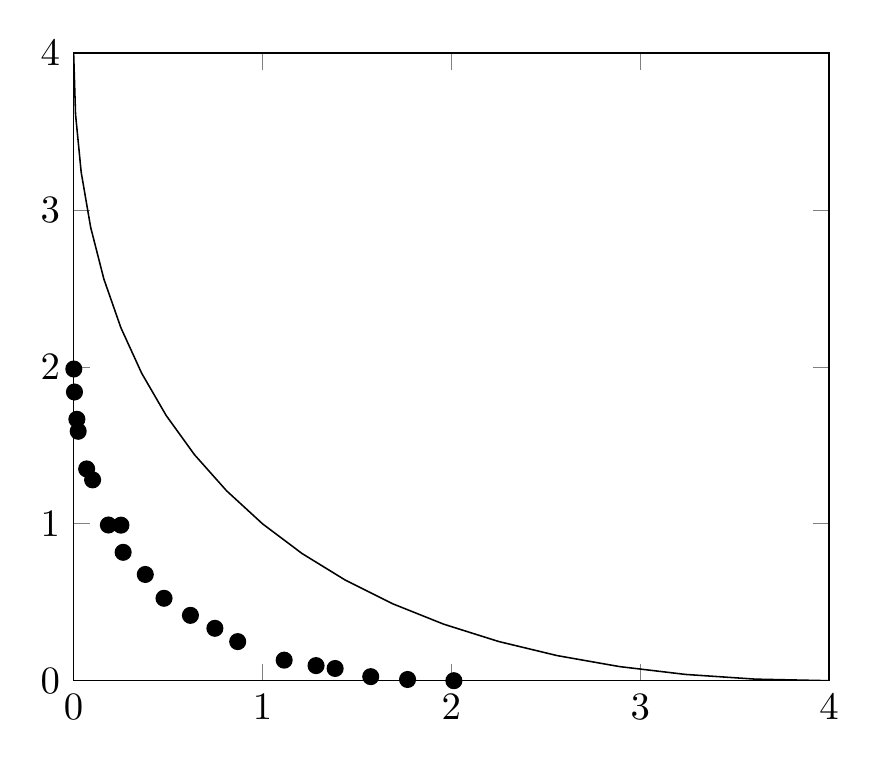
\begin{tikzpicture}[scale=1.4]
        \begin{axis}[enlargelimits=false]
            \addplot [] coordinates {
                (0.000000,4.000000) (0.010000,3.610000) (0.040000,3.240000) (0.090000,2.890000) (0.160000,2.560000) (0.250000,2.250000) (0.360000,1.960000) (0.490000,1.690000) (0.640000,1.440000) (0.810000,1.210000) (1.000000,1.000000) (1.210000,0.810000) (1.440000,0.640000) (1.690000,0.490000) (1.960000,0.360000) (2.250000,0.250000) (2.560000,0.160000) (2.890000,0.090000) (3.240000,0.040000) (3.610000,0.010000) (4.000000,0.000000) 
            };
            
            \addplot [only marks] coordinates {
                (2.013170,0.000022)(0.000811,1.986390)(1.114710,0.131126)(0.379304,0.677108)(0.478528,0.525250)(0.100382,1.280112)(1.767965,0.007815)(1.572890,0.025887)(0.262084,0.818221)(0.183932,0.992356)(0.868628,0.249256)(0.068938,1.349704)(0.024135,1.589631)(1.384435,0.078019)(0.004371,1.839921)(1.283436,0.096246)(0.618352,0.416527)(0.747836,0.333917)(0.017118,1.666182)(0.250461,0.991359) 
            };
        \end{axis}
    \end{tikzpicture}
\end{figure}